\documentclass[12pt]{article}
\usepackage{amsmath}
\usepackage{mathtext}
\usepackage[T2A]{fontenc}
\usepackage[utf8]{inputenc}
\usepackage[russian]{babel}
\usepackage[left=2cm, right=2cm, top=2.00cm]{geometry}
\usepackage[section]{placeins}

\title{Отчёт о выполнении лабораторной работы 1.2 <<Исследование эффекта Комптона>>}
\author{Маланчук С.В.}
% \author{Плохой Красный Коммунист}
\date{16.09.2020}

\usepackage{natbib}
\usepackage{graphicx}

\begin{document}

\begin{flushright}
    Выполнила:
    \\
    Маланчук С.В.,
    \\
    878 группа
    % \it{Плохой Красный Коммунист}
\end{flushright}

\begin{center}
    \begin{Large}
        \textbf{Отчёт о выполнении лабораторной работы 1.2 <<Исследование эффекта Комптона>>}
    \end{Large}
\end{center}

% \maketitle

\parindent=1cm \textbf{Цель работы:} исследовать энергетический спектр
$\gamma$-квантов, рассеянных на графите; определить энергию рассеянных квантов в
зависимости от угла рассеяния и энергию покоя частиц, на которых происходит рассеяние.

\parindent=1cm \textbf{Оборудование:} сцинтилляционный спектрометр; источник
излучения ($^{137}Cs$ в свинцовом контейнере с коллиматором); графитовая мишень.

\begin{center}
    \textbf{Теория}
\end{center}

Эффект Комптона~--- увеличение длны волны рассеянного света по сравнению с падающим.
\begin{equation}
    \label{eq:(1)}
    \Delta \lambda = \lambda_1 - \lambda_0 = \frac{h}{mc}(1 - \cos(\theta)) = \Lambda_K(1 - \cos(\theta))
\end{equation}
$\Lambda_K = \frac{h}{mc} = 2,42 \cdot 10^{-10} \text{см}$~--- комптоновская
длина волны электрона.
\begin{equation}
    \label{eq:(2)}
    \frac{1}{\varepsilon(\theta)} - \frac{1}{\varepsilon_0} = (1 - \cos(\theta))
\end{equation}
$\varepsilon_0 = \frac{E_0}{mc^2}$~--- энергия падающих $\gamma$-квантов,
$\varepsilon(\theta)$~--- испытавших рассеяние на угол $\theta$.
\begin{equation}
    \label{eq:(3)}
    \frac{1}{N(\theta)} - \frac{1}{N(0)} = A(1 - \cos(\theta))
\end{equation}
$N$~--- номер канала.
\begin{equation}
    \label{eq:(4)}
    mc^2 = E(0)\frac{E(90)}{E(0) - E(90)} = E_{\gamma} \frac{N(90)}{N(0) - N(90)}
\end{equation}
\newpage
\begin{center}
    \textbf{Ход работы}
\end{center}

\begin{center}
    \textbf{Измерения и наблюдения}
\end{center}

\begin{center}
    \begin{tabular}{|c|c|}
      \hline
      $\theta, ^\circ$ & $N(\theta)$ \\
      \hline           
      0 & 770  \\
      \hline           
      10 & 777 \\
      \hline           
      20 & 691 \\
      \hline           
      30 & 650 \\
      \hline           
      40 & 605 \\
      \hline           
      50 & 548 \\
      \hline           
      60 & 458 \\
      \hline           
      70 & 405 \\
      \hline           
      80 & 381 \\
      \hline           
      90 & 320 \\
      \hline           
      100 & 305 \\
      \hline           
      110 & 273 \\
      \hline           
      120 & 244 \\
      \hline           
    \end{tabular}
    % \caption{Видимость полос}
\end{center}
% \end{table}
\begin{center}
    \begin{tabular}{cc}
      \includegraphics[scale=0.4]{0.png} & 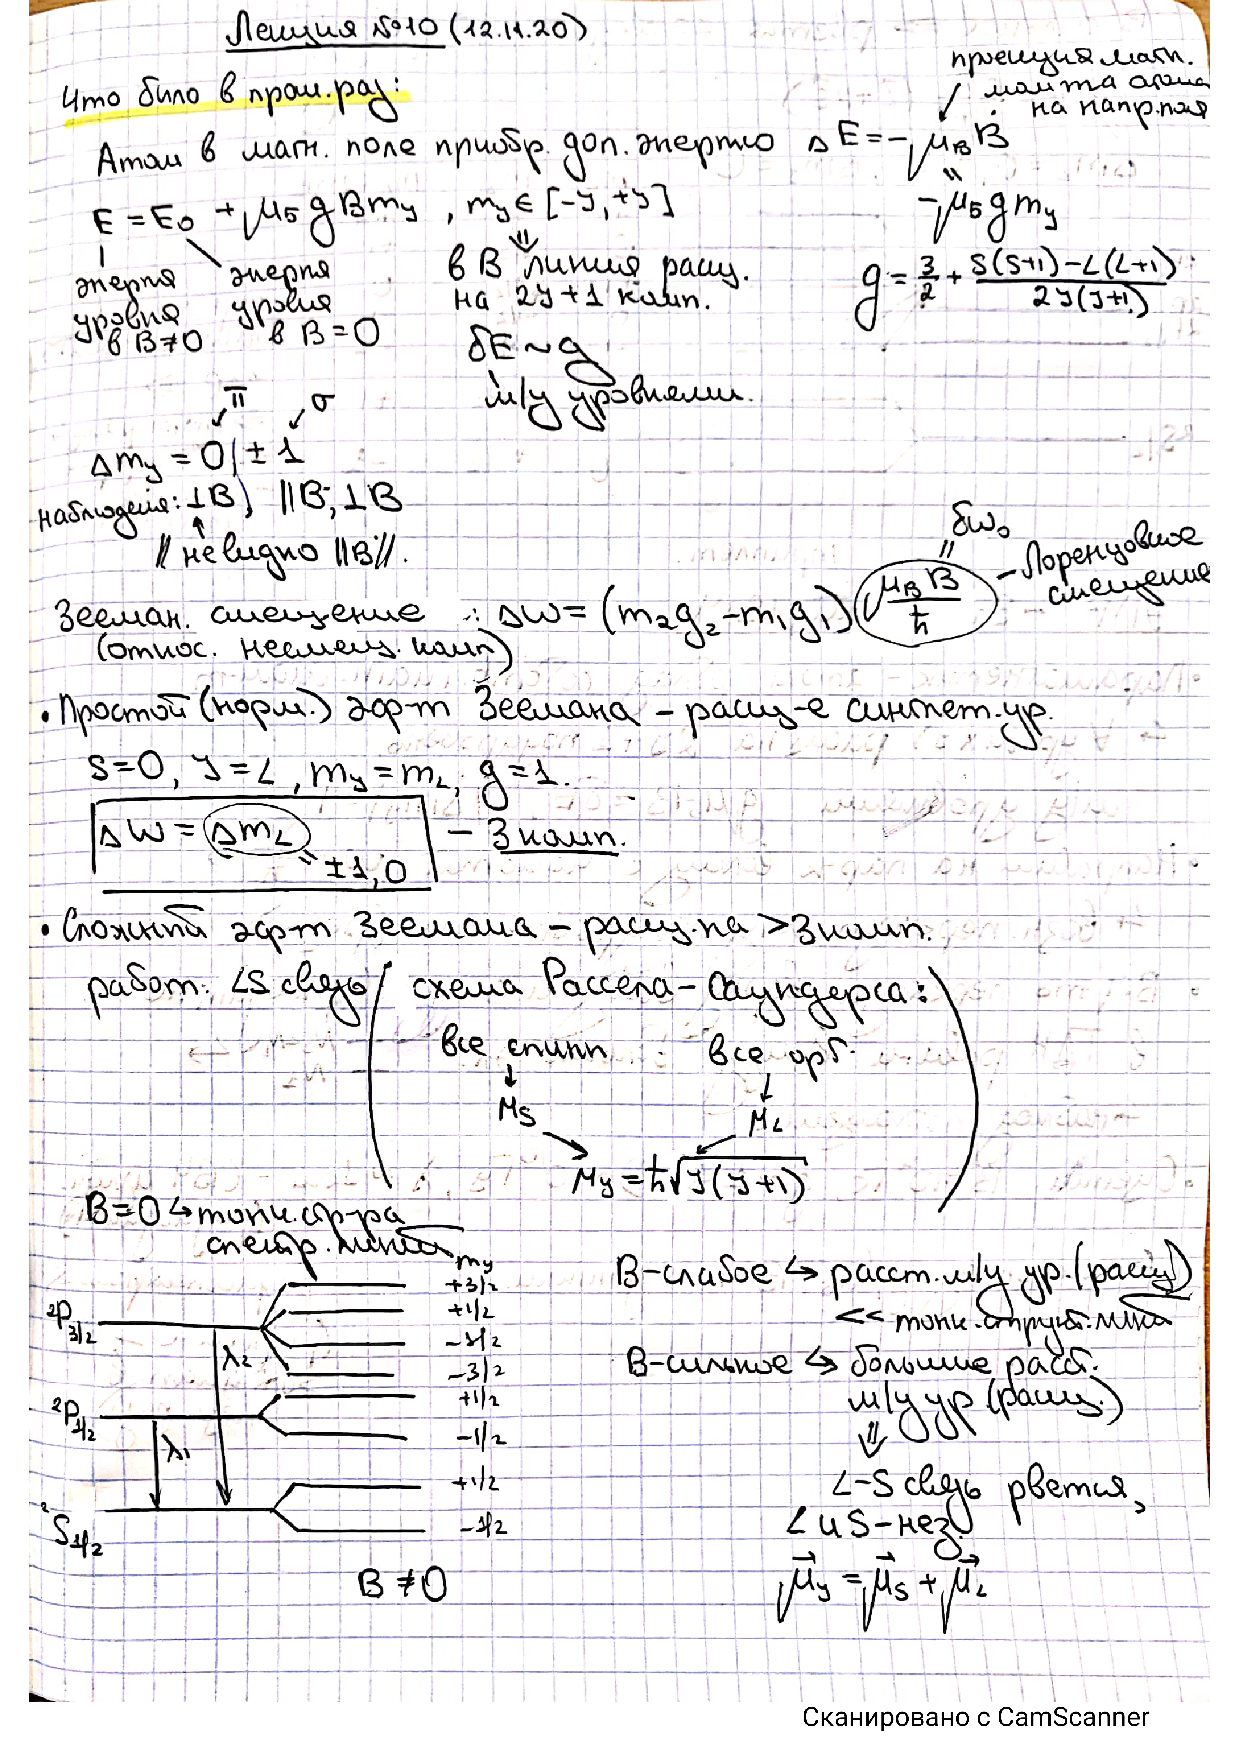
\includegraphics[scale=0.35]{10.png} \\
      \includegraphics[scale=0.37]{20.png} & \includegraphics[scale=0.35]{30.png} \\
    \end{tabular}
    % \caption{Видимость полос}
\end{center}
% \end{table}
\begin{center}
    \begin{tabular}{cc}
      \includegraphics[scale=0.35]{40.png} & \includegraphics[scale=0.35]{50.png} \\
      \includegraphics[scale=0.35]{60.png} & \includegraphics[scale=0.35]{70.png} \\
      \includegraphics[scale=0.35]{80.png} & \includegraphics[scale=0.35]{90.png} \\
    \end{tabular}
    % \caption{Видимость полос}
\end{center}
% \end{table}
\begin{center}
    \begin{tabular}{cc}
      \includegraphics[scale=0.35]{100.png} & \includegraphics[scale=0.35]{110.png} \\
    \end{tabular}
    % \caption{Видимость полос}
\end{center}
\begin{center}
    \includegraphics[scale=0.4]{120.png}
\end{center}
На изображениях показаны распределения, которые наблюдались в ходе эксперимента.
\\
Здесь можем видеть, как смещается пик.
\begin{center}
    \begin{tabular}{cc}
      \includegraphics[scale=0.35]{0_40.png} & \includegraphics[scale=0.35]{40_80.png} \\
    \end{tabular}
    % \caption{Видимость полос}
\end{center}
\begin{center}
    \includegraphics[scale=0.4]{80_120.png}
\end{center}
\begin{center}
    \textbf{Обработка}
\end{center}
\begin{center}
    \begin{tabular}{|c|c|c|c|c|c|c|c|c|c|}
      \hline
      $\theta, ^\circ$ & $\theta, rad$ & $N(\theta)$ & $1 - \cos(\theta)$ & $\frac{1}{N(\theta)}$ & $\sigma_\theta, rad$ & $\varepsilon_{N(\theta)}$ & $\sigma_{1 - \cos(\theta)}$ & $\sigma_{N(\theta)}$ & $\sigma_{\frac{1}{N(\theta)}}$ \\
      \hline
      0 & 0 & 770 & 0,0000 & 0,00130 & 0,009 & 0,01 & 0,0000 & 7,7 & 0,000013 \\
      \hline
      10 & 0,175 & 777 & 0,0152 & 0,00129 & 0,009 & 0,01 & 0,0047 & 7,77 & 0,000013 \\
      \hline
      20 & 0,349 & 691 & 0,0603 & 0,00145 & 0,009 & 0,01 & 0,0080 & 6,91 & 0,000014 \\
      \hline
      30 & 0,524 & 650 & 0,1340 & 0,00154 & 0,009 & 0,01 & 0,0086 & 6,5 & 0,000015 \\
      \hline
      40 & 0,698 & 605 & 0,2340 & 0,00165 & 0,009 & 0,01 & 0,0065 & 6,05 & 0,000017 \\
      \hline
      50 & 0,873 & 548 & 0,3572 & 0,00182 & 0,009 & 0,01 & 0,0023 & 5,48 & 0,000018 \\
      \hline
      60 & 1,047 & 458 & 0,5000 & 0,00218 & 0,009 & 0,01 & 0,0027 & 4,58 & 0,000022 \\
      \hline
      70 & 1,222 & 405 & 0,6580 & 0,00247 & 0,009 & 0,01 & 0,0068 & 4,05 & 0,000025 \\
      \hline
      80 & 1,396 & 381 & 0,8264 & 0,00262 & 0,009 & 0,01 & 0,0087 & 3,81 & 0,000026 \\
      \hline
      90 & 1,571 & 320 & 1,0000 & 0,00313 & 0,009 & 0,01 & 0,0078 & 3,2 & 0,000031 \\
      \hline
      100 & 1,745 & 305 & 1,1736 & 0,00328 & 0,009 & 0,01 & 0,0044 & 3,05 & 0,000033 \\
      \hline
      110 & 1,920 & 273 & 1,3420 & 0,00366 & 0,009 & 0,01 & 0,0004 & 2,73 & 0,000037 \\
      \hline
      120 & 2,094 & 244 & 1,5000 & 0,00410 & 0,009 & 0,01 & 0,0051 & 2,44 & 0,000041 \\
      \hline
    \end{tabular}
    % \caption{Видимость полос}
\end{center}
%Тогда
%$$E_{\gamma} = mc^2\frac{N(0) - N(90)}{N(90)} = (115 \pm 2,3)\cdot 10^{-15} =
%(1,15 \pm 0,2) \cdot 10^{-13} \text{Дж} = (7,2 \pm 1,2) \cdot 10^{4} \text{эВ}$$
%График см. на следующей странице.
%\newpage
\begin{figure}[ht!]
    \centering
    \includegraphics[scale=0.4]{plot1.png}
    \label{fig:plot1}
\end{figure}
Тогда
$$A = \frac{\frac{1}{N(\theta)} - \frac{1}{N(0)}}{1 - cos(\theta)}$$
Возьмем $\theta = 90^\circ$, значения $\displaystyle \frac{1}{N_{best}(90)} = 0,00305$ и
$\displaystyle \frac{1}{N_{best}(0)} = 0,00125$, тогда
$$A \approx 0,00180$$
$$\varepsilon_A = \varepsilon_{\frac{1}{N(90)} - \frac{1}{N(0)}} +
\varepsilon_{1 - cos(90^\circ)} = \frac{0,000044}{0,0043} + 0,0078 \approx
0,018$$
$$\sigma_A = 0,00003$$
$$A = (1,80 \pm 0,03) \cdot 10^{-3}$$
Тогда
$$\varepsilon_0 = AN(0) \approx 0,0018 \cdot 770 = 1,386$$
$$\varepsilon_{\varepsilon_0} = 0,018 + 0,01 = 0,028$$
$$\sigma_{\varepsilon_0} = 0,04$$
$$\varepsilon_0 = 1,39 \pm 0,04$$
%$$\varepsilon(90) = AN(90) = 0,0018 \cdot 320 = 0,576$$
Тогда энергия покоя (полагаем $E_0 \approx 600\text{кэВ}$)
$$mc^2 = \frac{E_0}{\varepsilon_0} \approx \frac{600}{1,39} \approx 432 \text{кэВ}$$
Полагая погрешность $E_0$ (табличного) равной нулю, имеем
$$\varepsilon_{mc^2} = 0,028$$
$$mc^2 = 432 \pm 12 \text{кэВ}$$
% \begin{figure}[ht!]
%     \centering
%     \includegraphics[scale=0.4]{plot1.png}
%     \caption{$\alpha = 0,033$}
%     \label{fig:plot1}
% \end{figure}
\begin{center}
    \textbf{Обсуждение}
\end{center}
Выполнив данную лабораторную работу, мы пронаблюдали сдвиг влево положения
фотопика при увеличении угла рассеяния; накладывая графики друг на друга, нашли
уровень вторичного рассеяния; установили значение энергии покоя частиц, на
которых происходит комптоновское рассеяние ($mc^2 = 432 \pm 12 \text{кэВ}$).
Значение совпало по порядку с табличным для электрона ($\approx 511
\text{кэВ}$), тем самым мы подтвердили тот факт, что рассеяние происходит на
электронах. Кроме того, пронаблюдали линейную зависимость $\displaystyle \frac{1}{N(\theta)}$ от $1 -
\cos \theta$.
\\
Также в ходе работы мы заметили важность использования свинцового экрана для
защиты счетчика от частиц, проникающих сквозь оболочку защитного контейнера:
провели эксперименты на больших углах дважды, значения с экраном лучше
соответствовали линейной зависимости.
\begin{center}
    \textbf{Вывод}
\end{center}
Энергия покоя частиц, на которых происходит комптоновское рассеяние: $mc^2 = 432
\pm 12 \text{кэВ}$. По порядку совпадает с табличным для электрона.
\end{document}
